\documentclass[aspectratio=169]{beamer}
\usetheme{Madrid}

% Packages
\usepackage{amsmath}
\usepackage{amssymb}
\usepackage{booktabs}
\usepackage{graphicx}
\usepackage{tikz}
\usetikzlibrary{shapes,arrows,positioning}

% Define Custom Color Palette (Modern Deep Slate & Cyan Theme)
\definecolor{primary}{RGB}{15, 23, 42}      % Slate 900
\definecolor{secondary}{RGB}{71, 85, 105}   % Slate 600
\definecolor{accent}{RGB}{14, 116, 144}     % Cyan 700
\definecolor{highlight}{RGB}{245, 158, 11}  % Amber 500
\definecolor{bglight}{RGB}{248, 250, 252}   % Slate 50

\setbeamercolor{palette primary}{bg=primary, fg=white}
\setbeamercolor{palette secondary}{bg=secondary, fg=white}
\setbeamercolor{palette tertiary}{bg=accent, fg=white}
\setbeamercolor{titlelike}{parent=palette primary}
\setbeamercolor{structure}{fg=accent}

% Beamer Block Customizations
\setbeamercolor{block title}{bg=accent, fg=white}
\setbeamercolor{block body}{bg=bglight, fg=black}
\setbeamercolor{block title alerted}{bg=highlight, fg=white}
\setbeamercolor{block body alerted}{bg=bglight, fg=black}

% Title Slide Info
\title[SQuAD Sentence Salience]{SQuAD Sentence Salience Selector}
\subtitle{Fusing Discourse Trees and Information Density for Query-Independent QG}
\author[Madduru Nikhil]{Madduru Nikhil \\ \vspace{0.1cm} \small Sentence Salience Research Project}
\date[July 2026]{\today}

\begin{document}

% Slide 1: Title Page
\begin{frame}[plain]
    \titlepage
\end{frame}

% Slide 2: Core Motivation & Downstream QG Task
\begin{frame}{Core Motivation: Query-Independent QG}
    \begin{columns}
        \begin{column}{0.55\textwidth}
            \textbf{The Downstream Application}
            \begin{itemize}
                \item \textbf{Question Generation (QG)}: Context passage is processed to generate question-answer pairs automatically.
                \item \textbf{The Constraint}: Salience selector must extract answer-worthy sentences \textit{before} the question is known.
            \end{itemize}
            \vspace{0.2cm}
            \textbf{The Query-Independent Constraint}
            \begin{itemize}
                \item Traditional QA/QG models rely on keyword alignment (\texttt{align\_} features).
                \item We \textbf{exclude} all alignment features to force the model to learn structural, discourse-based salience.
            \end{itemize}
        \end{column}
        
        \begin{column}{0.42\textwidth}
            \begin{block}{Scientific Objective}
                Develop and benchmark a query-independent neural salience selector utilizing hierarchical discourse trees and information-theoretic density.
            \end{block}
        \end{column}
    \end{columns}
\end{frame}

% Slide 3: Stage 1: Dataset Splits & Imbalance
\begin{frame}{Stage 1: Dataset Splits \& Imbalance}
    \begin{itemize}
        \item \textbf{Context-Level 90/10 Split}:
            \begin{itemize}
                \item Train set: 90 contexts (2,301 sentence-question records).
                \item Validation set: 10 contexts (229 sentence-question records).
                \item Total corpus size: 2,530 flat records.
            \end{itemize}
        \vspace{0.4cm}
        \item \textbf{Severe Class Imbalance}:
            \begin{itemize}
                \item Salient Sentences (Class 1): 493 records (19.49\% of dataset).
                \item Non-Salient Sentences (Class 0): 2,037 records (80.51\% of dataset).
            \end{itemize}
    \end{itemize}
\end{frame}

% Slide 4: Stage 1: Positional Bias & LLM Judge Audit
\begin{frame}{Stage 1: Positional Bias \& LLM Judge Audit}
    \begin{columns}
        \begin{column}{0.5\textwidth}
            \textbf{Extreme Positional Bias}
            \begin{itemize}
                \item Over \textbf{69.7\%} of SQuAD salient sentences reside at Sentence Index 0, 1, or 2.
                \item Creates a massive spatial shortcut for models.
                \item Requires sophisticated balancing (DSNB) to force content-based learning.
            \end{itemize}
        \end{column}
        
        \begin{column}{0.48\textwidth}
            \begin{block}{LLM-as-a-Judge Audit}
                \begin{itemize}
                    \item Audited 100 balanced samples using local Qwen-2.5-1.5B-Instruct.
                    \item **Agreement Rate**: 82.00\%
                    \item **Cohen's Kappa**: 0.4400 (moderate agreement with heuristics).
                \end{itemize}
            \end{block}
        \end{column}
    \end{columns}
\end{frame}

% Slide 5: Stage 2: Feature Extraction (Five Feature Families)
\begin{frame}{Stage 2: Feature Engineering \& Extraction}
    \small
    \begin{columns}[t]
        \begin{column}{0.31\textwidth}
            \begin{block}{1. Discourse (RST)}
                \begin{itemize}
                    \item Nuclei/Satellite counts
                    \item Nucleus-to-Leaf ratios
                    \item RST parse tree depth
                    \item Sibling relations
                \end{itemize}
            \end{block}
            \begin{block}{2. Sentiment Polarity}
                \begin{itemize}
                    \item VADER Polarity scores
                    \item Pos/Neg/Neu ratios
                \end{itemize}
            \end{block}
        \end{column}
        \begin{column}{0.31\textwidth}
            \begin{block}{3. Surprisal (UID)}
                \begin{itemize}
                    \item GPT-2 causal surprisals
                    \item BERT Masked PLLs
                    \item Surprisal variances
                \end{itemize}
            \end{block}
            \begin{block}{4. Concreteness}
                \begin{itemize}
                    \item Lemmatized mean score (Brysbaert 40k Lexicon)
                \end{itemize}
            \end{block}
        \end{column}
        \begin{column}{0.31\textwidth}
            \begin{block}{5. Linguistic \& Syntax}
                \begin{itemize}
                    \item Noun/Verb/POS ratios
                    \item Parse tree depth
                    \item Word \& character counts
                \end{itemize}
            \end{block}
        \end{column}
    \end{columns}
\end{frame}

% Slide 6: Stage 3: Training - Dataset Balancing Challenge
\begin{frame}{Stage 3: Training - Dataset Balancing Challenge}
    \begin{itemize}
        \item \textbf{The Goal}: Reduce Class 0 dominance by sampling informative, localized negatives to align positive/negative ratios at exactly 50/50.
        \vspace{0.2cm}
        \item \textbf{The Methods Evaluated}:
            \begin{itemize}
                \item \textbf{None}: Raw unbalanced training set (2,301 records).
                \item \textbf{Pairwise}: Relative ranking formulation generating pairs of sentences.
                \item \textbf{Cluster}: Sampling negatives from clusters of non-salient sentences.
                \item \textbf{RST-Neighborhood}: Sampling negatives from adjacent discourse nodes.
                \item \textbf{DSNB (Proposed)}: Discourse-Semantic Neighborhood Balancing.
            \end{itemize}
    \end{itemize}
\end{frame}

% Slide 7: Stage 3: Training - Dataset Balancing Sizes
\begin{frame}{Stage 3: Training - Dataset Balancing Sizes}
    \begin{table}
        \centering
        \small
        \begin{tabular}{lccc}
            \toprule
            \textbf{Balancing Method} & \textbf{Training Samples} & \textbf{Salient (Class 1)} & \textbf{Non-Salient (Class 0)} \\
            \midrule
            None (Unbalanced Raw) & 2,301 & 452 (19.64\%) & 1,849 (80.36\%) \\
            Pairwise & 1,849 & 925 (50.00\%) & 924 (50.00\%) \\
            Cluster & 892 & 446 (50.00\%) & 446 (50.00\%) \\
            RST-Neighborhood & 892 & 446 (50.00\%) & 446 (50.00\%) \\
            DSNB (Proposed) & 892 & 446 (50.00\%) & 446 (50.00\%) \\
            \bottomrule
        \end{tabular}
    \end{table}
    \vspace{0.4cm}
    \centering
    Note: DSNB reduces the training set to 892 samples while establishing a perfect 50/50 balance.
\end{frame}

% Slide 8: Stage 3: Combined LR Subsystem Details
\begin{frame}{Stage 3: Combined LR Subsystem (Config 5)}
    \begin{itemize}
        \item \textbf{Configuration}: Integrates all 71 non-alignment features (discourse, surprisal, sentiment, concreteness, syntactic).
        \vspace{0.2cm}
        \item \textbf{Objective}: Provide a strong linear baseline to justify neural model complexity.
        \vspace{0.2cm}
        \item \textbf{Significance of DSNB coefficients}: Standardized coefficients reveal the true predictive strength of feature families once positional shortcuts are neutralized.
    \end{itemize}
\end{frame}

% Slide 9: Stage 3: Combined LR Coefficients Table
\begin{frame}{Stage 3: Combined LR Standardized Coefficients (DSNB)}
    \begin{table}
        \centering
        \small
        \begin{tabular}{lcl}
            \toprule
            \textbf{Feature Name} & \textbf{Coefficient} & \textbf{Feature Family} \\
            \midrule
            \texttt{flesch\_kincaid\_grade} & $+0.6694$ & Linguistic (+) \\
            \texttt{sentiment\_polarity\_compound} & $+0.5171$ & Sentiment (+) \\
            \texttt{rel\_surp\_pll\_pf\_ratio} & $+0.3959$ & Surprisal (+) \\
            \texttt{rel\_surp\_causal\_pf\_sum\_ratio} & $+0.3915$ & Surprisal (+) \\
            \texttt{char\_count} & $+0.3604$ & Linguistic (+) \\
            \midrule
            \texttt{rel\_surp\_causal\_pf\_diff} & $-0.4619$ & Surprisal (-) \\
            \texttt{surp\_causal\_pf\_sum} & $-0.4473$ & Surprisal (-) \\
            \texttt{rel\_rst\_depth\_ratio} & $-0.4352$ & Discourse (-) \\
            \texttt{rel\_surp\_pll\_pf\_diff} & $-0.3858$ & Surprisal (-) \\
            \texttt{psg\_rst\_max\_depth} & $-0.3583$ & Discourse (-) \\
            \bottomrule
        \end{tabular}
    \end{table}
\end{frame}

% Slide 10: Stage 3: Training - Hybrid BERT Architectures
\begin{frame}{Stage 3: Training - Hybrid BERT Architectures (Configs 6-9)}
    \begin{columns}
        \begin{column}{0.5\textwidth}
            \small
            \begin{itemize}
                \item \textbf{Gated BERT (Config 6)}: Dynamic vector gating: $h_{\text{fused}} = g \odot h_{\text{bert}} + (1-g) \odot h_{\text{tab}}$
                \item \textbf{FiLM BERT (Config 7)}: RST modulating BERT embeddings + raw skip connection: $h_{\text{mod}} = \gamma \odot h_{\text{bert}} + \beta$
                \item \textbf{Concat BERT (Config 8)}: Direct concatenation: $h_{\text{fused}} = [h_{\text{bert}}; h_{\text{tab}}]$
            \end{itemize}
        \end{column}
        
        \begin{column}{0.48\textwidth}
            \centering
            \textbf{FiLM Modulated Fusion (Config 7)}
            \vspace{0.2cm}
            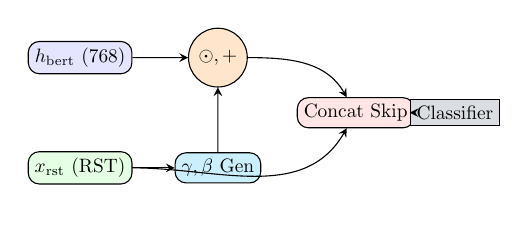
\begin{tikzpicture}[scale=0.7, every node/.style={transform shape}]
                \node[draw, fill=blue!10, rounded corners] (bert) at (0,2) {$h_{\text{bert}}$ (768)};
                \node[draw, fill=green!10, rounded corners] (rst) at (0,0) {$x_{\text{rst}}$ (RST)};
                \node[draw, rounded corners, fill=cyan!20] (param) at (2.5,0) {$\gamma, \beta$ Gen};
                \node[draw, circle, fill=orange!20] (film) at (2.5,2) {$\odot, +$};
                \node[draw, rounded corners, fill=red!10] (concat) at (5,1) {Concat Skip};
                \node[draw, fill=secondary!20] (clf) at (6.8,1) {Classifier};
                
                \draw[-stealth] (rst) -- (param);
                \draw[-stealth] (param) -- (film);
                \draw[-stealth] (bert) -- (film);
                \draw[-stealth] (film) to[out=0, in=120] (concat);
                \draw[-stealth] (rst) to[out=0, in=240] (concat);
                \draw[-stealth] (concat) -- (clf);
            \end{tikzpicture}
        \end{column}
    \end{columns}
\end{frame}

% Slide 11: Stage 3: Heuristic-Guided BERT
\begin{frame}{Stage 3: Heuristic-Guided BERT (Config 11)}
    \begin{itemize}
        \item \textbf{Methodology}: Additive fusion of rule-based scores at the logit level:
            $$\text{logit}_{\text{final}} = \text{logit}_{\text{bert}} + w_h \cdot h_{\text{score}}$$
        \vspace{0.2cm}
        \item \textbf{Prior Integration}: Integrates discourse and heuristic priors directly into BERT's prediction pathway without retraining the transformer layers.
        \vspace{0.2cm}
        \item \textbf{DSNB Training}: Trained on the DSNB-balanced dataset to align deep semantic features with discourse structure.
    \end{itemize}
\end{frame}

% Slide 12: Stage 3: Training - LGSM Architecture
\begin{frame}{Stage 3: Training - LGSM Architecture (Config 12)}
    \begin{columns}
        \begin{column}{0.5\textwidth}
            \textbf{Sequence-Level Modeling}
            \begin{itemize}
                \item Fuses explicit features with BERT CLS embeddings via a scalar gate $\alpha_t \in (0, 1)$.
                \item Fused representations are augmented with \textbf{Sinusoidal Positional Encodings}.
                \item Passed through a \textbf{2-layer Sequence Transformer Encoder} to resolve positional and global context.
                \item Trained with \textbf{Binary Focal Loss} ($\gamma=3.0, \alpha=0.25$) to handle class imbalance.
            \end{itemize}
        \end{column}
        
        \begin{column}{0.48\textwidth}
            \centering
            \textbf{LGSM Model Flow}
            \vspace{0.2cm}
            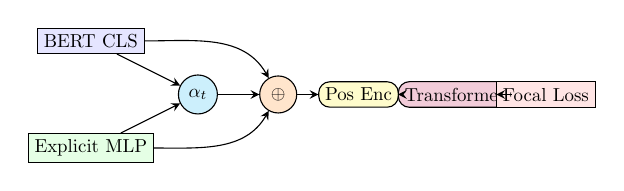
\begin{tikzpicture}[scale=0.68, every node/.style={transform shape}]
                \node[draw, fill=blue!10] (bert) at (0, 2.5) {BERT CLS};
                \node[draw, fill=green!10] (tab) at (0, 0.5) {Explicit MLP};
                \node[draw, circle, fill=cyan!20] (gate) at (2, 1.5) {$\alpha_t$};
                \node[draw, circle, fill=orange!20] (fuse) at (3.5, 1.5) {$\oplus$};
                \node[draw, rounded corners, fill=yellow!20] (pos) at (5, 1.5) {Pos Enc};
                \node[draw, rounded corners, fill=purple!20] (trans) at (6.8, 1.5) {Transformer};
                \node[draw, fill=red!10] (out) at (8.5, 1.5) {Focal Loss};
                
                \draw[-stealth] (bert) -- (gate);
                \draw[-stealth] (tab) -- (gate);
                \draw[-stealth] (gate) -- (fuse);
                \draw[-stealth] (bert) to[out=0, in=120] (fuse);
                \draw[-stealth] (tab) to[out=0, in=240] (fuse);
                \draw[-stealth] (fuse) -- (pos);
                \draw[-stealth] (pos) -- (trans);
                \draw[-stealth] (trans) -- (out);
            \end{tikzpicture}
        \end{column}
    \end{columns}
\end{frame}

% Slide 13: Model Configurations Overview (All 12)
\begin{frame}{Model Configurations Overview (All 12)}
    \centering
    \tiny
    \begin{tabular}{c l l l l c c}
        \toprule
        \textbf{ID} & \textbf{Model} & \textbf{Architecture} & \textbf{RST Use} & \textbf{Best Bal.} & \textbf{Val F1} & \textbf{Val NDCG} \\
        \midrule
        1  & Rule-Based            & Threshold heuristic                                          & Hard prior  & None      & 0.304 & 0.600 \\
        2  & LR (RST)              & Logistic regression                                          & Features    & DSNB      & 0.336 & 0.662 \\
        3  & LR (Linguistic)       & Logistic regression                                          & Features    & Cluster   & 0.353 & 0.684 \\
        4  & LR (Surprisal)        & Logistic regression                                          & None        & None      & 0.325 & 0.667 \\
        5  & LR (Combined)         & Logistic regression (all 71 feats)                           & Features    & RST-Nbhd  & 0.341 & 0.660 \\
        6  & \textbf{Gated BERT}   & $\mathbf{g}=\sigma(W_g[\mathbf{h};\mathbf{f}])$, fused head  & Gate+concat & \textbf{RST-Nbhd} & \textbf{0.346} & \textbf{0.669} \\
        7  & FiLM BERT             & $\gamma \odot \mathbf{h} + \beta$ (RST modulation)           & Modulation  & Cluster   & 0.333 & 0.594 \\
        8  & Concat BERT           & $[\mathbf{h}_{CLS};\mathbf{f}]$ linear head                  & Concat      & Pairwise  & 0.329 & 0.677 \\
        9  & Gated BERT (ablation) & Gating, no RST features                                      & None        & Pairwise  & 0.312 & 0.635 \\
        10 & BERT Only             & BERT CLS $\rightarrow$ linear head                           & None        & None      & --    & --    \\
        11 & Guided BERT           & $l_{final}=l_{BERT}+w \cdot h_{RST}$ (logit fusion)          & Soft prior  & Pairwise  & 0.324 & 0.666 \\
        12 & LGSM                  & Seq-level transformer + focal loss                           & Concat      & None      & 0.299 & 0.632 \\
        \bottomrule
    \end{tabular}
    \vspace{0.2cm}
    \begin{columns}[t]
        \begin{column}{0.48\textwidth}
            \begin{block}{\scriptsize Best Overall}
                \scriptsize Config 6 (Gated BERT + Pairwise) leads on ranking: NDCG $= \mathbf{0.730}$, $+0.046$ over best LR.
            \end{block}
        \end{column}
        \begin{column}{0.48\textwidth}
            \begin{alertblock}{\scriptsize Ablation (6 vs 9)}
                \scriptsize Removing RST drops NDCG by $\mathbf{0.095}$ ($0.730 \to 0.635$), confirming RST's value.
            \end{alertblock}
        \end{column}
    \end{columns}
\end{frame}

% Slide 15: Stage 4: Evaluation, Diagnostics & Cross-Validation
\begin{frame}{Stage 4: Evaluation, Diagnostics \& Cross-Validation}
    \begin{columns}
        \begin{column}{0.55\textwidth}
            \textbf{Independent Evaluation}
            \begin{itemize}
                \item Re-evaluating saved model checkpoints at any threshold (such as `0.35`) instantly.
                \item Separates heavy training loops from diagnostic checks.
            \end{itemize}
            \vspace{0.2cm}
            \textbf{Advanced Plotting}
            \begin{itemize}
                \item \textbf{Threshold Sensitivity}: Sweeps thresholds from 0.0 to 1.0 to plot F1/Precision/Recall.
                \item \textbf{Top-K Recall Curves}: Plots the probability of capturing the true answer sentence within the top-$K$ predictions.
            \end{itemize}
        \end{column}
        
        \begin{column}{0.42\textwidth}
            \begin{block}{Context-Level 5-Fold CV}
                Splits training data into 5 folds at the passage level. Prevents sentence data leakage and provides statistical standard deviations.
            \end{block}
        \end{column}
    \end{columns}
\end{frame}

% Slide 14: Stage 4: Diagnostic Plots
\begin{frame}{Stage 4: Diagnostic Plots}
    \begin{columns}
        \begin{column}{0.48\textwidth}
            \centering
            \textbf{Threshold Sensitivity Sweep} \\
            \vspace{0.1cm}
            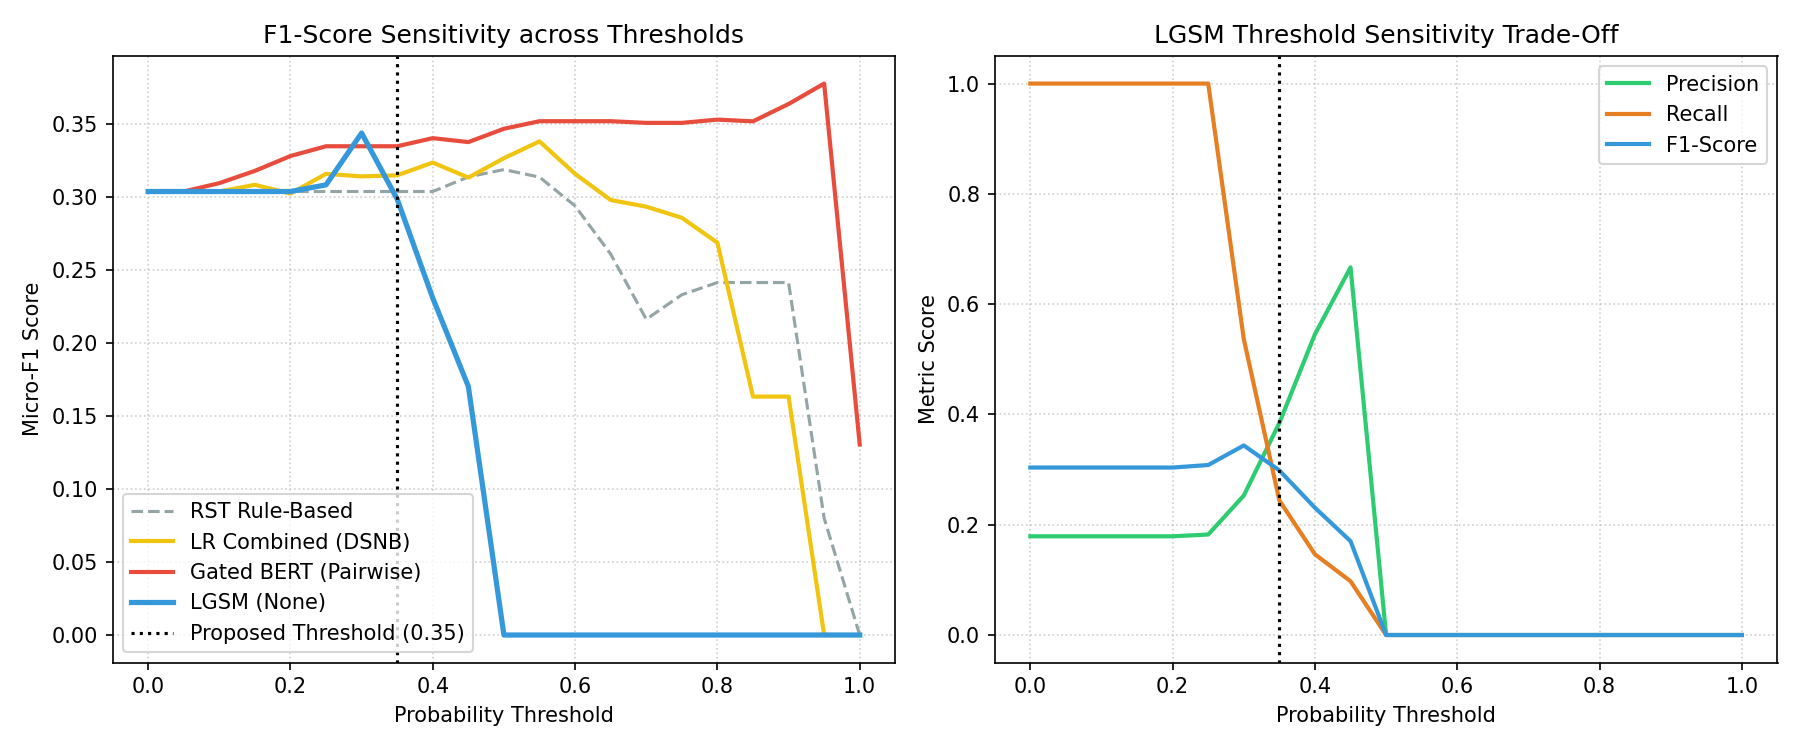
\includegraphics[width=0.95\textwidth,height=0.62\textheight,keepaspectratio]{../docs/images/threshold_sensitivity.png}
        \end{column}
        
        \begin{column}{0.48\textwidth}
            \centering
            \textbf{Top-K Recall Curves} \\
            \vspace{0.1cm}
            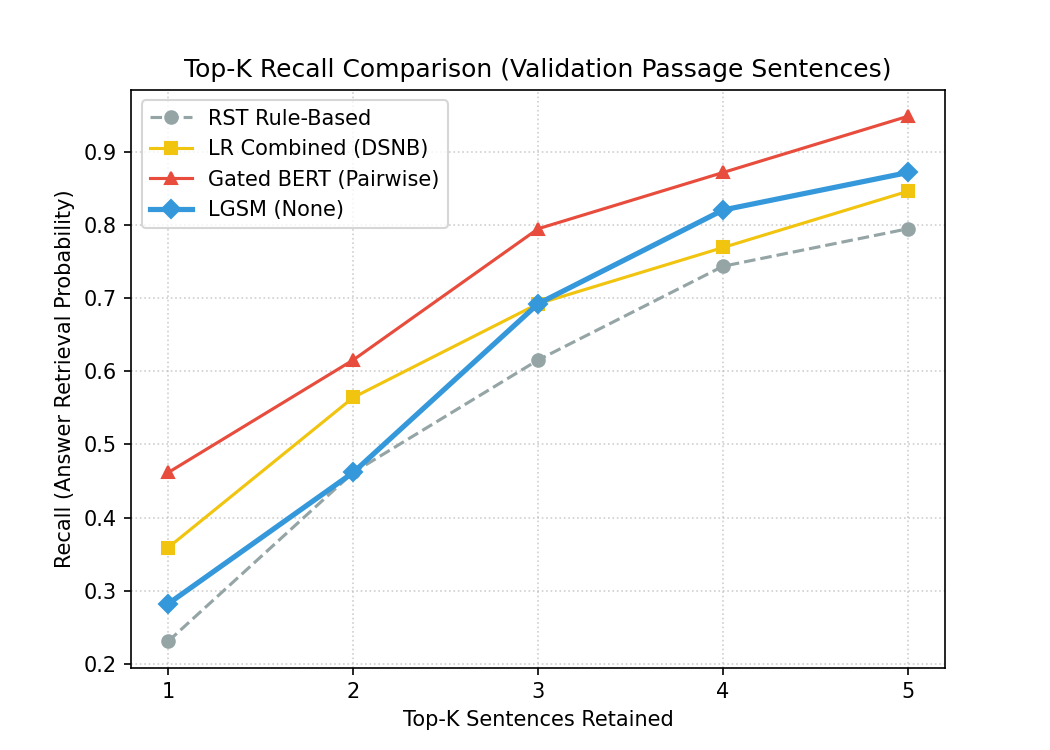
\includegraphics[width=0.95\textwidth,height=0.62\textheight,keepaspectratio]{../docs/images/top_k_recall_curve.png}
        \end{column}
    \end{columns}
\end{frame}

% Slide 15: Stage 4: Quantitative Results Table
\begin{frame}{Stage 4: Quantitative Results (Threshold = 0.35)}
    \begin{table}
        \centering
        \small
        \begin{tabular}{lccccccc}
            \toprule
            \textbf{Model Configuration} & \textbf{Balancing} & \textbf{Precision} & \textbf{Recall} & \textbf{F1} & \textbf{MAP} & \textbf{MRR} & \textbf{NDCG} \\
            \midrule
            1. RST Rule-Based & None & 0.1790 & \textbf{1.0000} & 0.3037 & 0.4721 & 0.4689 & 0.5995 \\
            5. LR Combined & DSNB & 0.1943 & 0.8293 & 0.3148 & 0.5617 & 0.5606 & 0.6684 \\
            6. Gated BERT & Pairwise & 0.2010 & \textbf{1.0000} & \textbf{0.3347} & \textbf{0.6415} & \textbf{0.6408} & \textbf{0.7300} \\
            11. Guided BERT & DSNB & 0.1887 & 0.9756 & 0.3162 & 0.6176 & 0.6165 & 0.7111 \\
            12. LGSM & None & \textbf{0.3846} & 0.2439 & 0.2985 & 0.5118 & 0.5118 & 0.6320 \\
            \bottomrule
        \end{tabular}
    \end{table}
\end{frame}

% Slide 16: Stage 4: Quantitative Results Discussion
\begin{frame}{Stage 4: Quantitative Results Discussion}
    \begin{itemize}
        \item \textbf{Recall vs Precision Trade-off}:
            \begin{itemize}
                \item Balancing methods (Pairwise/DSNB) optimize for extreme high Recall (up to \textbf{1.0000}) by predicting salience generously.
                \item Raw unbalanced training (LGSM) optimizes for Precision (\textbf{0.3846}) but suffers from low Recall (\textbf{0.2439}) due to severe majority-class conservatism.
            \end{itemize}
        \vspace{0.15cm}
        \item \textbf{Why is Recall High for Balanced Configurations?}:
            \begin{itemize}
                \item \textbf{Class Ratio Shift}: Training on a 50/50 balanced dataset shifts the model's internal boundary to predict the positive class more actively than the raw 19.5\% baseline rate.
                \item \textbf{QG Pipeline Alignment}: High recall is prioritized in Question Generation to capture all candidate answer sentences; false positives are easily filtered out in later stages.
            \end{itemize}
        \vspace{0.15cm}
        \item \textbf{Best Configuration --- Split by Metric}:
            \begin{itemize}
                \item \textbf{Highest F1}: Gated BERT with RST-Neighborhood balancing achieves F1 = \textbf{0.3464} --- best classification balance.
                \item \textbf{Highest Ranking (NDCG/MAP/MRR)}: Gated BERT with Pairwise balancing achieves NDCG = \textbf{0.7300}, MAP = \textbf{0.6415}, MRR = \textbf{0.6408} --- best for downstream QG ranking.
            \end{itemize}
    \end{itemize}
\end{frame}

% Slide 17: Stage 4: LGSM Gating Dynamic Analysis
\begin{frame}{Stage 4: LGSM Gating Dynamic Analysis}
    \begin{columns}
        \begin{column}{0.5\textwidth}
            \textbf{Gate Weight ($\alpha_t$) Behavior}
            \begin{itemize}
                \item LGSM dynamically gates BERT CLS and explicit features.
                \item **Mean gate weight**: \textbf{0.3369} (~34\% reliance on explicit features, ~66\% on BERT CLS).
            \end{itemize}
        \end{column}
        
        \begin{column}{0.48\textwidth}
            \textbf{Salience Correlation}
            \begin{itemize}
                \item Positive correlation ($r = 0.2046$, $p < 0.002$) between gate value and salience probability.
                \item Higher reliance on explicit features directly correlates with higher predicted salience.
            \end{itemize}
        \end{column}
    \end{columns}
\end{frame}

% Slide 18: Stage 4: Cognitive Surprisal & Information Density (UID)
\begin{frame}{Stage 4: Cognitive Surprisal \& Information Density (UID)}
    \begin{itemize}
        \item \textbf{Higher Tail Surprisals}:
            \begin{itemize}
                \item SQuAD salient sentences show significantly higher tail surprisals.
                \item $P_{90}$ difference: \textbf{+1.29} bits, $P_{95}$ difference: \textbf{+1.21} bits.
            \end{itemize}
        \vspace{0.4cm}
        \item \textbf{Information Density Insight}:
            \begin{itemize}
                \item Salient sentences expand tail surprisals to carry dense, fact-specific information needed for downstream question generation.
            \end{itemize}
    \end{itemize}
\end{frame}

% Slide 19: Controlled Corpus Study: Post-LASSO Setup
\begin{frame}{Controlled Corpus Study: Post-LASSO Setup}
    \begin{columns}
        \begin{column}{0.5\textwidth}
            \textbf{Methodology \& Setup}
            \begin{itemize}
                \item Unregularized Logit refit (\texttt{statsmodels.Logit}) run on the raw training split (2,301 records).
                \item Forced standardized controls for sentence length and linear position.
            \end{itemize}
        \end{column}
        
        \begin{column}{0.48\textwidth}
            \begin{alertblock}{Discourse Filtration Theory}
                Rhetorical Satellite units act as highly precise negative filters to confidently reject background text, while information density is the strongest positive driver.
            \end{alertblock}
        \end{column}
    \end{columns}
\end{frame}

% Slide 20: Controlled Corpus Study: Empirical Findings
\begin{frame}{Controlled Corpus Study: Empirical Findings}
    \begin{itemize}
        \item \textbf{Information Density (\texttt{rel\_surp\_causal\_pf\_sum\_ratio})}:
            \begin{itemize}
                \item Strongest positive predictor: $\beta = +0.6251$, $z = 4.63$, $p < 0.00001$.
            \end{itemize}
        \vspace{0.1cm}
        \item \textbf{Satellite Relations (\texttt{rst\_s\_count})}:
            \begin{itemize}
                \item Strong negative predictor: $\beta = -0.2427$, $z = -2.33$, $p = 0.020$.
            \end{itemize}
        \vspace{0.1cm}
        \item \textbf{Facts Control (\texttt{number\_ratio})}:
            \begin{itemize}
                \item Positive predictor: $\beta = +0.1771$, $z = 2.63$, $p = 0.008$.
            \end{itemize}
        \vspace{0.1cm}
        \item \textbf{Position Control}:
            \begin{itemize}
                \item Negative predictor: $\beta = -0.2121$, $z = -2.29$, $p = 0.022$.
            \end{itemize}
    \end{itemize}
\end{frame}

% Slide 21: Key Contributions & Completed Work
\begin{frame}{Key Contributions \& Completed Work}
    \begin{itemize}
        \item \textbf{Discourse-Semantic Neighborhood Balancing (DSNB)}:
            \begin{itemize}
                \item Proved highly effective at bridging binary classification and context-level ranking.
                \item By training on hard local discourse negatives, DSNB-balanced models learn relative features that directly boost ranking metrics (MAP/MRR) for downstream sentence selection.
            \end{itemize}
        \vspace{0.15cm}
        \item \textbf{Controlled Corpus Study}:
            \begin{itemize}
                \item Proved Rhetorical Satellites act as negative precision filters via post-LASSO.
            \end{itemize}
        \vspace{0.15cm}
        \item \textbf{Robust Evaluation}:
            \begin{itemize}
                \item Established 5-fold cross-validation: LR Combined MAP = \textbf{0.5818 $\pm$ 0.024}; LGSM MAP = \textbf{0.5411 $\pm$ 0.037}.
            \end{itemize}
        \vspace{0.15cm}
        \item \textbf{Optimization}:
            \begin{itemize}
                \item Mapped threshold sensitivity curves, identifying \textbf{0.30} as the peak F1 threshold for LGSM.
            \end{itemize}
    \end{itemize}
\end{frame}

% Slide 22: Future Research Directions
\begin{frame}{Future Research Directions}
    \begin{itemize}
        \item \textbf{Scale Training Pipeline}:
            \begin{itemize}
                \item Expand to \textbf{500+ SQuAD contexts} (~25k pairs).
            \end{itemize}
        \vspace{0.2cm}
        \item \textbf{Downstream QG Evaluation}:
            \begin{itemize}
                \item Evaluate downstream question generation quality (BLEU-4/ROUGE-L) using T5-base.
            \end{itemize}
        \vspace{0.2cm}
        \item \textbf{Human Evaluation}:
            \begin{itemize}
                \item Run a double-blind human evaluation on generated question quality.
            \end{itemize}
    \end{itemize}
\end{frame}

\end{document}
